\documentclass[11pt]{article}

\usepackage[a4paper,margin=26mm]{geometry}
\usepackage[T1]{fontenc}
\usepackage[utf8]{inputenc}
\usepackage{lmodern}
\usepackage{microtype}
\usepackage{amsmath,amssymb,mathtools}
\usepackage{booktabs}
\usepackage{enumitem}
\usepackage{graphicx}
\usepackage[round,authoryear]{natbib}
\usepackage[hidelinks]{hyperref}
\hypersetup{
  pdftitle={Capability and Observability Effects in Value-Bundle Inference},
  pdfauthor={Gunnar Zarncke},
  pdfsubject={Value-bundle inference, observability, and capability geometry}
}

\setlist{nosep,leftmargin=*}
\setlength{\parindent}{1.2em}
\setlength{\parskip}{0.25em}

\newcommand{\E}{\mathbb{E}}
\newcommand{\Pp}{\mathbb{P}}
\newcommand{\R}{\mathbb{R}}
\newcommand{\I}{\mathcal{I}}
\newcommand{\C}{\mathcal{C}}
\newcommand{\V}{\mathcal{V}}
\newcommand{\Reach}{\mathcal{R}}
\newcommand{\KL}{D_{\mathrm{KL}}}
\newcommand{\doop}{\mathrm{do}}

\title{\textbf{Capability and Observability Effects in Value-Bundle Inference}\\
\large Why Viable Systems Can Look Similar While Failures Look Distinct}
\author{Gunnar Zarncke}
\date{October 2026}

\begin{document}
\maketitle

\begin{abstract}
Value learning from behavior faces a structural ambiguity: the dimensions that are easiest to infer from observations need not be the dimensions that causally organize successful behavior. We develop this point for a \emph{value-bundle} model in which values are relatively low-dimensional regulatory constraints or control directions embedded in a much higher-dimensional behavioral state space. Two effects interact. First, an \emph{observability effect}: positive or norm-conforming attributes may be frequent and mutually similar, whereas negative deviations are rarer and more heterogeneous. Cognitive-ecological work shows that this ecology makes negative attributes disproportionately distinctive and therefore disproportionately useful for differentiating persons and groups \citep{AlvesKochUnkelbach2017Common,AlvesKochUnkelbach2017Good,AlvesKochUnkelbach2018,UnkelbachKochAlves2019,UnkelbachWeitzelAlves2026}. Second, a \emph{capability effect}: successful regulation can preserve a large set of feasible actions and future trajectories even when the constraints defining success are few, whereas heterogeneous failures can each collapse the system into a comparatively narrow region of reachable state space. Hence ``good is alike'' in diagnostic or constraint coordinates can coexist with ``good is diverse'' in behavioral and capability coordinates. We formalize this as a distinction between low-dimensional value coordinates $B$, high-dimensional diagnostic residuals $R$, and a capability functional measuring the viable reachable set. The resulting capability--observability inversion explains why observational learning can overrepresent negative distinctions, why diagnostic information is not equivalent to normative or causal importance, and why value learning should attempt to recover invariant regulatory structure rather than simply the features that best discriminate observed behavior. The framework connects cognitive-ecological valence asymmetries, viability and control theory, resilience, biological degeneracy, empowerment, homeostatic reinforcement learning, and inverse reinforcement learning.
\end{abstract}

\section{Introduction}

Suppose an observer attempts to infer what a person, institution, culture, or artificial agent values from its behavior. A natural assumption is that the most characteristic observations are also the most revealing observations: if some feature strongly distinguishes one agent from another, then that feature should receive substantial weight in the inferred representation of their values. This assumption is attractive but generally false. Statistical distinctiveness concerns the geometry of the \emph{observation channel}; value concerns the causal organization of the \emph{controlled system}. The two geometries need not coincide.

A particularly useful case is provided by recent work on evaluative information ecologies. Positive social attributes tend to be more frequent, while negative attributes tend to be more diverse. Positive attributes are therefore relatively likely to be shared, while negative attributes are relatively likely to differentiate targets \citep{AlvesKochUnkelbach2017Common,AlvesKochUnkelbach2017Good,UnkelbachKochAlves2019}. Alves, Koch, and Unkelbach \citeyearpar{AlvesKochUnkelbach2018} showed how this ecological structure can generate negative impressions of novel groups without requiring an independent motivational preference for derogation. More recently, \citet{UnkelbachWeitzelAlves2026} formalize the implication for stereotypes: if perceivers characterize groups through attributes that distinguish them from other groups, and negative attributes are simultaneously less frequent and more diverse, characteristic group attributes will tend to be negative. Rare attributes may consequently be highly diagnostic of group membership even when they describe only a minority of the group's members.

This result has a direct but nontrivial implication for models of value inference. The naive interpretation is that negative value content is intrinsically more differentiated than positive value content. We propose a different interpretation. Negative observations may be more differentiated because they encode \emph{which constraint failed}, whereas successful regulation suppresses precisely those deviations. A relatively compact set of maintained constraints can therefore generate a large number of distinguishable failure modes. Conversely, satisfying those constraints can preserve a very large set of actions, strategies, and trajectories. Thus the same system can exhibit
\begin{equation}
    \text{low diagnostic diversity under success}
    \quad\text{and}\quad
    \text{high behavioral diversity under success},
\end{equation}
while exhibiting
\begin{equation}
    \text{high diagnostic diversity under failure}
    \quad\text{and}\quad
    \text{low capability under failure}.
\end{equation}

This distinction resolves an apparent tension in the familiar Tolstoyan intuition that successful systems are alike whereas unsuccessful systems fail in different ways. If ``diversity'' means diversity of \emph{failure signatures}, the intuition is plausible. If diversity instead means the number of viable trajectories available to the system, the ordering may reverse. Healthy organisms, competent institutions, functional families, and robust artificial agents can satisfy a comparatively small set of invariants while retaining enormous behavioral freedom. Dysfunction may reveal many different violated invariants while simultaneously reducing what the system can actually do.

We call this reversal the \emph{capability--observability inversion}. It matters for value learning because observations are sampled in behavioral coordinates, while the object to be inferred may live in regulatory coordinates. A learner that compresses observations according to variance, prediction error, distinctiveness, or mutual information can therefore allocate disproportionate representational capacity to heterogeneous failures. It may learn an ontology of cruelty, corruption, neglect, domination, betrayal, recklessness, rigidity, and exclusion even if these are better understood as heterogeneous residuals generated by violations of a smaller set of regulatory bundles such as care, fairness, epistemic integrity, autonomy, or reciprocity.

The claim is not that such negative concepts are unreal, reducible in every case, or normatively unimportant. It is that \emph{observational dimensionality does not identify causal dimensionality}. The number of phenomenologically or linguistically distinct ways to violate a value need not equal the number of independent values required to explain regulation.

\section{Value Bundles as Regulatory Coordinates}

Let the environment have latent state
\[
    x_t \in \mathcal{X},
\]
with actions $a_t\in\mathcal{A}(x_t)$ and dynamics
\[
    x_{t+1}\sim P(\cdot\mid x_t,a_t).
\]
The learner does not necessarily observe $x_t$ directly. Instead,
\[
    y_t\sim O_\eta(\cdot\mid x_t,a_t),
\]
where $O_\eta$ denotes an observation channel determined by perceptual access, measurement choices, social salience, reporting practices, and the broader information ecology.

We represent the agent's value organization by
\[
    \Theta=(B,W,\Phi).
\]
Here $B=(b_1,\ldots,b_k)$ denotes a collection of latent \emph{value bundles}, $W$ their context-sensitive relative control strengths, and $\Phi$ their \emph{bearer maps}: functions determining which persons, entities, time horizons, or portions of the world fall under a bundle's scope. The important assumption is not that $B$ consists of familiar moral labels. It is that $k$ may be much smaller than the dimensionality of raw behavior.

A standard inverse-choice model might write
\begin{equation}
 P(B,W,\Phi\mid A,I)
 \propto
 P(A\mid I,B,W,\Phi)P(B,W,\Phi),
 \label{eq:basicinverse}
\end{equation}
where $I$ is contextual information. Classical inverse reinforcement learning similarly attempts to recover a reward representation from observed behavior \citep{NgRussell2000}, while cooperative inverse reinforcement learning makes the inferential relationship between learner and demonstrator itself strategic \citep{HadfieldMenell2016}.

The value-bundle view departs from a simple reward-coordinate interpretation in one important respect. A bundle need not specify a desired point in state space. It may instead specify a \emph{maintained region}, invariant, inequality, or regulatory relation. Let
\begin{equation}
    \V_B
    =
    \left\{
       x\in\mathcal{X}:
       g_j(x;\,b_j,\phi_j)\leq 0,\;
       j=1,\ldots,k
    \right\}
    \label{eq:viableset}
\end{equation}
be the region compatible with the active bundles. The system regulates so as to remain within, return toward, or enlarge its controllable region inside $\V_B$.

This interpretation connects naturally to cybernetic and viability-theoretic views of regulation. Ashby's law of requisite variety emphasizes that successful regulation requires sufficient control variety relative to disturbances \citep{Ashby1956}; Conant and Ashby's good-regulator theorem links effective regulation to internal models of the regulated system \citep{ConantAshby1970}; viability theory studies the states from which a system can remain within an admissible set under appropriate controls \citep{Aubin1991}. Homeostatic reinforcement learning similarly treats behavior as serving the regulation of internal variables rather than as merely maximizing arbitrary instantaneous rewards \citep{KeramatiGutkin2014}.

The conceptual shift is consequential. If a value is represented by a constraint, many superficially different behaviors can satisfy it. ``Care,'' for example, does not identify a unique action. Depending on state, resources, competence, recipient, and competing constraints, care can imply feeding, teaching, leaving alone, protecting, warning, forgiving, restraining, redistributing resources, or doing nothing. The commonality lies not necessarily in action-space similarity but in the regulatory relation preserved across contexts.

\section{The Ecological Asymmetry of Observable Evidence}

Let an observable attribute $F_i$ have valence $v_i\in\{+,-\}$. The cognitive-ecological literature distinguishes two statistical properties:
\begin{align}
    \Pp(F_i=1\mid v_i=+) &>
    \Pp(F_i=1\mid v_i=-)
    &&\text{(positivity prevalence)},\\
    |\mathcal{F}_{-}| &>
    |\mathcal{F}_{+}|
    &&\text{(negativity diversity)}.
\end{align}
The second inequality should not be interpreted merely as a dictionary count. It states that negative information can occupy a larger or more heterogeneous region of feature space. One proposed source is a range structure in which an acceptable intermediate region is flanked by multiple undesirable extremes: too little and too much can both be bad, while a narrower middle range is satisfactory \citep{AlvesKochUnkelbach2017Good,UnkelbachKochAlves2019}.

Positivity prevalence alone already implies that positive attributes are more likely to be shared. If two independently sampled targets possess feature $i$ with probability $p_i$, the probability of sharing its presence is $p_i^2$. High-prevalence features therefore contribute disproportionately to commonality. If negative attributes are additionally distributed over a larger vocabulary, the realized negative feature of one target is less likely to match the realized negative feature of another.

For group differentiation, what matters is not valence itself but diagnosticity. For a group variable $G$ and observation $F$,
\begin{equation}
    \I(G;F)
    =
    \E\left[
      \log
      \frac{P(F\mid G)}{P(F)}
    \right].
    \label{eq:mutualinfo}
\end{equation}
A rare feature can carry large information about $G$ when its conditional prevalence differs sharply across groups. In pointwise form,
\begin{equation}
    i(g;f)
    =
    \log
    \frac{P(f\mid g)}{P(f)}.
\end{equation}
Thus rarity is not by itself diagnosticity, but rarity combined with group-specific concentration can produce high diagnostic information. This qualification matters: the ecological argument does not license the inference that every rare negative feature is informative. It predicts a distributional tendency under conditions where negative attributes are spread more heterogeneously across targets.

The ``common good'' phenomenon follows from this structure: similarities tend to be positive and differences negative \citep{AlvesKochUnkelbach2017Common}. The later intergroup work demonstrates that when novel groups are represented disproportionately through unique features, the valence asymmetry of those unique features can generate evaluative disadvantage \citep{AlvesKochUnkelbach2018}. The 2026 theory extends the argument to characteristic stereotype content \citep{UnkelbachWeitzelAlves2026}.

For value inference, the key lesson is more general:
\begin{equation}
    \boxed{
    \text{features useful for identification}
    \neq
    \text{features constitutive of the underlying controller}.
    }
    \label{eq:identification}
\end{equation}
A symptom can identify a disease without being its cause; a fault code can identify a subsystem without being the system's objective; and a distinctive norm violation can identify a group or individual without corresponding to an independent negative value.

\section{Capability Geometry}

We now introduce a second geometry. Let
\begin{equation}
 \Reach_H(x)
 =
 \left\{
 x_{t+H}:
 \exists\,a_{t:t+H-1}
 \text{ with nonzero transition probability from }x
 \right\}
\end{equation}
be the $H$-step reachable set. Given value bundle $B$, define the \emph{viable reachable set}
\begin{equation}
 \Reach_H^{B}(x)
 =
 \left\{
 x_{t+H}\in\Reach_H(x):
 x_{t+\tau}\in\V_B
 \text{ for }0\leq\tau\leq H
 \right\}.
\end{equation}
A simple capability functional is
\begin{equation}
    \C_H(x;B)
    =
    \log \mu\!\left(\Reach_H^{B}(x)\right),
    \label{eq:capvolume}
\end{equation}
for an appropriate measure $\mu$. In discrete spaces, $\mu$ may simply count reachable states. More sophisticated definitions can weight reachable outcomes by quality, robustness, controllability, or bearer-specific accessibility.

An information-theoretic analogue is empowerment, defined through the channel capacity from action sequences to future sensory or world states \citep{KlyubinPolaniNehaniv2005}:
\begin{equation}
    \mathcal{E}_H(x)
    =
    \max_{p(a_{t:t+H-1})}
    I(A_{t:t+H-1};X_{t+H}\mid X_t=x).
    \label{eq:empowerment}
\end{equation}
Both \eqref{eq:capvolume} and \eqref{eq:empowerment} capture the intuition that possessing many distinguishable, controllable futures is a form of capability.

The important fact is that constraints need not reduce capability monotonically. A local constraint can preserve the global conditions under which many future options remain possible. Avoiding catastrophic injury constrains immediate action but preserves future mobility. Epistemic discipline forbids convenient falsehoods but preserves the reliability of later inference. Reciprocity restricts exploitative strategies but can preserve cooperative relationships and future exchange. Constitutional constraints remove some political actions while maintaining a broader space of stable social coordination.

Thus a small number of maintained invariants may act as \emph{option-preserving constraints}. This is closely related to resilience: persistence is not identical to constancy but concerns the ability of a system to absorb disturbance without losing its organizing regime \citep{Holling1973}. Biological degeneracy provides a complementary mechanism. Structurally different components or pathways can perform overlapping functions, allowing the same functional constraint to be satisfied through heterogeneous implementations \citep{EdelmanGally2001}. Functional invariance and behavioral diversity are therefore entirely compatible.

The geometry is approximately
\begin{equation}
\boxed{
\begin{array}{c}
\text{few maintained constraints}\\[2pt]
\Downarrow\\[2pt]
\text{large viable manifold}\\[2pt]
\Downarrow\\[2pt]
\text{many admissible policies and trajectories}.
\end{array}}
\label{eq:capgeometry}
\end{equation}
The dimensionality of the constraint description can be low even when the intrinsic dimensionality or entropy of the admissible behavior is high.

\section{Failure Residuals}

Let
\begin{equation}
    r_j(x)
    =
    [g_j(x)]_+
    =
    \max\{0,g_j(x)\}
\end{equation}
measure violation of constraint $j$, and let
\[
    R(x)=(r_1(x),\ldots,r_m(x),\rho(x))
\]
collect observable residuals, where $\rho$ may include downstream symptoms produced by the violations.

The decomposition relevant for value inference is then
\begin{equation}
    z_t=g_\psi(y_{\leq t},a_{<t})
    =
    (B_t,R_t),
    \label{eq:decomposition}
\end{equation}
where $B_t$ represents inferred regulatory structure and $R_t$ represents diagnostic deviation from that structure.

The dimensions need not be equal. Indeed, we hypothesize
\begin{equation}
    \dim_{\mathrm{eff}}(B)
    \ll
    \dim_{\mathrm{eff}}(R)
    \lesssim
    \dim_{\mathrm{eff}}(Y).
    \label{eq:rank}
\end{equation}
A single maintained constraint can fail through many causal chains and produce many observable syndromes. ``Preserve epistemic integrity,'' for example, can fail through fabrication, motivated reasoning, selective omission, source laundering, overconfidence, strategic ambiguity, confabulation, or deference to unreliable authority. These observations may be usefully distinguished even if they are not independent terminal values.

This produces an Anna Karenina-like structure without requiring a metaphysically larger set of negative values. Let success require $k$ approximately conjunctive conditions,
\begin{equation}
    S
    =
    \bigcap_{j=1}^{k}
    \{g_j(x)\leq 0\}.
\end{equation}
Failure is its complement,
\begin{equation}
    S^c
    =
    \bigcup_{j=1}^{k}
    \{g_j(x)>0\}.
    \label{eq:unionfail}
\end{equation}
The successful region is defined by simultaneous satisfaction of constraints, while failure decomposes into a union of distinct violation regions and their intersections. Even with only $k$ constraints, there are up to $2^k-1$ nonempty patterns of violated subsets. Additional causal and contextual variation can subdivide each pattern further.

Consequently, the number of diagnostic categories can grow combinatorially while the regulatory description remains compact. This yields
\begin{equation}
    H(R\mid \text{failure})
    >
    H(R\mid \text{successful regulation})
    \label{eq:residualentropy}
\end{equation}
under broad conditions, because successful regulation drives residuals toward a common low-error region.

Yet \eqref{eq:residualentropy} says nothing about the entropy of actions or trajectories. We may simultaneously have
\begin{equation}
    H(A_{t:t+H}\mid \text{success})
    >
    H(A_{t:t+H}\mid \text{failure}),
    \label{eq:actionentropy}
\end{equation}
or, more substantively,
\begin{equation}
    \E[\C_H(X_t;B)\mid\text{success}]
    >
    \E[\C_H(X_t;B)\mid\text{failure}].
    \label{eq:capinversion}
\end{equation}
Equations \eqref{eq:residualentropy} and \eqref{eq:capinversion} constitute the core inversion: failure can be more diverse as a \emph{diagnosis} while success is more diverse as a \emph{capacity for action}.

\section{Capability--Observability Inversion}

We can state the argument as a stylized proposition.

\paragraph{Proposition 1 (Capability--observability inversion).}
Suppose that (i) successful regulation requires satisfaction of a compact collection of viability constraints; (ii) different constraint violations generate distinguishable residual signatures; (iii) at least some violations remove actions, resources, controllability, or reachable states; and (iv) observations encode deviations from regulated variables more distinctly than ordinary within-viability variation. Then it is possible, and under these assumptions natural, for
\begin{align}
    H(R\mid F=1) &> H(R\mid F=0),\\
    \E[\C_H(X)\mid F=1] &< \E[\C_H(X)\mid F=0],
\end{align}
where $F=1$ denotes regulatory failure.

The result is not a mathematical theorem about all systems; each assumption can be violated. It is instead a structural pattern. A machine in working order may perform thousands of tasks while emitting the same ``normal'' status signal. Its failures may have dozens of distinct error codes, although each error reduces what the machine can do. A healthy organism can occupy a vast behavioral repertoire while maintaining body temperature, blood gases, glucose, and other regulated variables inside comparatively narrow ranges. Pathology may create diagnostically rich deviations precisely while reducing mobility, cognition, endurance, or behavioral flexibility. A functioning institution can support heterogeneous projects under a small set of procedural invariants; corruption, capture, paralysis, arbitrary enforcement, and factional breakdown are distinct failures that each contract the institution's effective action space.

Thus the statement ``there are more ways to be bad than good'' is coordinate-dependent. In residual coordinates it can be true:
\[
    |\mathcal{R}_{\mathrm{bad}}|
    \gg
    |\mathcal{R}_{\mathrm{good}}|.
\]
In policy or trajectory coordinates, the reverse can hold:
\[
    |\Pi_{\mathrm{viable}}|
    \gg
    |\Pi_{\mathrm{failed}}|.
\]
No contradiction follows because the maps between these spaces are many-to-one.

\section{Observability Is Not Normative Importance}

The preceding argument becomes important when a learner constructs latent representations from observations. Let $Z=(B,R)$. The information made available by observation channel $O_\eta$ about a latent coordinate $Z_j$ is
\begin{equation}
    \I_\eta(Z_j;Y\mid I)
    =
    \E\left[
    \log
    \frac{p_\eta(Y\mid Z_j,I)}
         {p_\eta(Y\mid I)}
    \right].
    \label{eq:obsinfo}
\end{equation}
Learning procedures driven by prediction, compression, discrimination, reconstruction, or likelihood will generally prefer latent directions that explain observable variance. If negative residuals are rare, heterogeneous, and identity-diagnostic, they can have high marginal information value.

A value learner can therefore encounter
\begin{equation}
    \I(R;Y)
    \gg
    \I(B;Y)
\end{equation}
even when $B$ is causally upstream of $R$. This is especially likely when successful regulation makes $B$ observationally quiet. A thermostat's set point is least visible when regulation works perfectly; the set point becomes inferable from perturbation and correction. Likewise, a norm continuously satisfied by almost everyone can be statistically unhelpful for differentiating people while being indispensable to the organization of the social system.

Define the causal-regulatory importance of bundle coordinate $b_j$ by the change in future viable capability under intervention,
\begin{equation}
    K_j
    =
    \E\left[
      \C_H(X_{t+H};B)
      -
      \C_H(X_{t+H};B^{(j,\delta)})
      \,\middle|\,
      \doop(b_j\leftarrow b_j+\delta)
    \right],
    \label{eq:causalimportance}
\end{equation}
or by another interventionally defined loss functional. There is no general reason for
\begin{equation}
    \arg\max_j \I(Z_j;Y)
    =
    \arg\max_j K_j.
    \label{eq:argmax}
\end{equation}
Indeed, the capability--observability inversion predicts systematic disagreement.

Equation \eqref{eq:argmax} is the central warning for observational value learning:
\begin{equation}
\boxed{
    \text{diagnostic information}
    \not\equiv
    \text{causal importance}
    \not\equiv
    \text{normative importance}.
}
\end{equation}
Mutual information is symmetric and observational. Value regulation is directional and causal. Normative importance introduces a further question---what should be preserved---which cannot in general be recovered merely by ranking observable features according to statistical informativeness.

\section{Why Negative Concepts Can Dominate Learned Ontologies}

Suppose a representation learner receives behavioral data from many agents and minimizes
\begin{equation}
    \mathcal{L}
    =
    \mathcal{L}_{\mathrm{pred}}
    +
    \lambda\mathcal{L}_{\mathrm{recon}}
    +
    \beta\Omega(z),
\end{equation}
where $\Omega$ penalizes representational complexity. If most positive behavior is common across agents, encoding fine distinctions among positive observations yields little improvement in prediction of agent identity. Distinct negative residuals, by contrast, can sharply reduce uncertainty. Under a fixed representation budget, the learner may therefore allocate dimensions to negative residual categories.

This yields an \emph{observational overdecomposition} of failure:
\begin{equation}
    B
    \longrightarrow
    \begin{cases}
       R_1\\
       R_2\\
       \vdots\\
       R_m
    \end{cases}
    \longrightarrow Y,
    \qquad
    m\gg k,
\end{equation}
followed by a learned ontology that mistakes $\{R_1,\ldots,R_m\}$ for independent motivational primitives.

The error is analogous to inferring the objective function of an engineered controller from its alarm vocabulary. An aircraft may have separate alarms for low oil pressure, excessive turbine temperature, hydraulic failure, icing, stall, sensor disagreement, and fuel imbalance. The diversity of alarms is not evidence that the aircraft has an equally large set of independent ``negative goals.'' Alarm diversity reflects the combinatorics of ways in which a smaller collection of operating requirements can be violated.

Human moral vocabulary may contain a related mixture. Terms such as betrayal, abandonment, exploitation, favoritism, humiliation, coercion, corruption, negligence, recklessness, fanaticism, and hypocrisy can be psychologically and socially real categories while nevertheless being partly organized as failure residuals around lower-rank regulatory bundles. A value ontology learned purely from lexical or behavioral variance would tend to assign these categories more independent structure than it assigns ubiquitous successful regulation.

This prediction is strengthened by the evaluative information ecology. If positive behavior is both prevalent and similar, successful value expression is statistically compressed before the learner even begins. Negative behavior arrives pre-separated into distinctive clusters.

\section{Bearer Maps and Boundary Observations}

The effect is particularly strong for bearer maps. Let
\begin{equation}
    \phi_j(z_{\mathrm{world}})
    \in [0,1]
\end{equation}
denote the extent to which bundle $b_j$ applies to a candidate bearer in world state $z_{\mathrm{world}}$. A person may endorse care, fairness, autonomy, or reciprocity while varying dramatically in the entities to whom the principle is applied.

Ordinary positive behavior toward canonical bearers is weak evidence about the boundary of $\phi_j$. If nearly everyone protects their own children, avoids gratuitous harm to friends, and honors reciprocal obligations within a familiar community, those observations provide limited discriminatory information. Boundary cases are more revealing:
\begin{equation}
    \text{outsider},\quad
    \text{enemy},\quad
    \text{criminal},\quad
    \text{nonhuman animal},\quad
    \text{future person},\quad
    \text{distant stranger}.
\end{equation}
Selective refusal or extension of concern in such cases can sharply constrain the inferred bearer map.

Hence negative or conflictual cases may legitimately be \emph{epistemically} privileged. The mistake would be to infer from this epistemic privilege that exclusion itself is the fundamental value coordinate. What is often identified is a \emph{boundary condition} on a more general bundle.

This suggests that difficult moral cases are useful for value inference for approximately the same reason adversarial examples and system-identification perturbations are useful in engineering: they excite otherwise latent dimensions of the controller. Their value is experimental, not necessarily ontological.

\section{Constraint Rank and Behavioral Rank}

The distinction can be sharpened using local dimensionality. Let a successful region be defined by $k$ independent active constraints in an $n$-dimensional state space,
\begin{equation}
    g_j(x)=0,
    \qquad j=1,\ldots,k,
\end{equation}
with Jacobian
\[
    J_g(x)
    =
    \frac{\partial(g_1,\ldots,g_k)}
         {\partial x}.
\]
If $\operatorname{rank}J_g=k<n$, then the locally admissible manifold has dimension approximately
\begin{equation}
    \dim\V_B=n-k.
\end{equation}
A \emph{low-rank control description} is therefore compatible with a \emph{high-dimensional behavioral manifold}. In fact, when $k\ll n$,
\[
    n-k\approx n.
\]
A small number of constraints can leave most degrees of freedom available.

Failure observations behave differently. Moving away from the viable manifold generates a normal component
\begin{equation}
    \delta x_\perp
    \in
    \operatorname{span}\{\nabla g_1,\ldots,\nabla g_k\},
\end{equation}
but downstream nonlinear dynamics can amplify and differentiate the consequences of that displacement. Different violated constraints, combinations of violations, temporal orders, compensatory responses, and contexts can yield a large family of observable residuals.

Thus ``high-dimensional content, low effective control rank'' is not paradoxical. The content of moral life can be extraordinarily rich because values operate over high-dimensional states, histories, relationships, and bearer maps, while the number of regulatory directions required to organize that content can remain much smaller.

\section{Resilience, Degeneracy, and Freedom Under Constraint}

The capability perspective also changes the intuitive relationship between normativity and freedom. If values are represented as point targets, adding values appears to add restrictions: each objective narrows the set of acceptable states. But regulatory constraints can be \emph{enabling constraints}. They exclude locally available actions that would destroy the preconditions for larger future action spaces.

Let
\begin{equation}
    \Delta\C_H(a\mid x)
    =
    \E[\C_H(X_{t+1};B)\mid x,a]
    -
    \C_H(x;B).
\end{equation}
An action can have high immediate reward while satisfying
\[
    \Delta\C_H(a\mid x)\ll0,
\]
thereby consuming future option value. Conversely, costly regulation can maintain or increase capability.

This is closely related to results showing that, across broad classes of reward functions, optimal policies can exhibit incentives to preserve access to future states or options \citep{TurnerEtAl2021}. The normative interpretation here is different: capability preservation is not automatically morally good, since an agent may preserve options for harmful purposes. Nevertheless, the mathematics illustrates why continued controllability is instrumentally valuable across many objectives.

Resilience and degeneracy add a further layer. A resilient system need not return to one microscopic state. It may preserve macroscopic organization while varying its implementation \citep{Holling1973}. Degenerate biological systems can reach the same functional outcome through structurally different components \citep{EdelmanGally2001}. A value bundle can similarly specify an invariant at one level while allowing diversity below it:
\begin{equation}
    \text{one regulatory equivalence class}
    \longleftarrow
    \text{many behavioral realizations}.
\end{equation}
Successful value expression should therefore not be expected to look behaviorally homogeneous once context and capability are adequately observed.

\section{Implications for Inverse Value Learning}

Standard inverse reinforcement learning already faces severe identifiability problems: multiple reward functions can rationalize the same policy \citep{NgRussell2000}. Capability--observability effects introduce a complementary problem. Even when behavior is informative, it may be informative primarily about residual structure rather than about the latent regulatory basis.

A more appropriate inference target is
\begin{align}
&P(B,W,\Phi,R_{1:T},X_{1:T}\mid
Y_{1:T},A_{1:T},I)
\nonumber\\
&\qquad\propto
P(B,W,\Phi)
\prod_{t=1}^{T}
O_\eta(y_t\mid x_t,a_t)
P(a_t\mid x_t,B,W,\Phi,R_t)
P(x_{t+1}\mid x_t,a_t)
P(R_t\mid x_t,B,\Phi).
\label{eq:fullmodel}
\end{align}
The decomposition forces the learner to distinguish three questions:
\begin{enumerate}[nosep,leftmargin=1.5em]
    \item What variables or relations appear to be regulated?
    \item How and where does regulation fail?
    \item Which entities and contexts fall inside the scope of the regulation?
\end{enumerate}

The model should not assume that residuals are valueless noise. Residual structure is crucial for identifying bundle boundaries and for predicting behavior under perturbation. The claim is instead that residuals and bundles play different explanatory roles.

An effective learner should therefore exploit \emph{interventions}, natural experiments, context variation, recovery trajectories, and counterfactual behavior. If a latent coordinate represents a genuine regulatory bundle, its signature should appear not merely in which failures occur but in how the system responds when pushed away from the viable region. Regulation is revealed by correction.

For a candidate variable $q(x)$, define regulatory evidence through expected corrective drift:
\begin{equation}
    \Gamma_q(x)
    =
    -\E[
       q(X_{t+1})-q(X_t)
       \mid q(X_t)\text{ displaced},\,I
    ].
\end{equation}
A variable with systematic restoring dynamics has stronger evidence of being controlled than a variable that merely covaries with identity. This provides one operational route for separating value bundles from descriptive traits.

\section{Observational Selection Effects}

The observation process itself may further amplify the asymmetry. Social observers, institutions, media, datasets, and evaluators do not sample behavior uniformly. Let
\begin{equation}
    S_t\in\{0,1\}
\end{equation}
indicate whether event $t$ enters the learner's dataset, with
\begin{equation}
    P(S_t=1\mid y_t)
\end{equation}
depending on novelty, severity, conflict, reportability, or institutional relevance. The effective training distribution is
\begin{equation}
    p_{\mathrm{obs}}(y)
    \propto
    p(y)P(S=1\mid y).
\end{equation}
Even modest selection toward unusual events can greatly increase the apparent prevalence of failure residuals.

This matters because successful regulation is often uneventful. A bridge that remains standing, a promise that is quietly kept, a database that preserves integrity, a caregiver who reliably meets ordinary needs, or an institution that processes thousands of cases procedurally may generate little individually memorable evidence. Violations generate records.

Hence the learner can face two multiplicative biases:
\begin{equation}
\underbrace{\text{ecological distinctiveness}}_{\substack{\text{negative features}\\\text{rarer and more diverse}}}
\times
\underbrace{\text{sampling distinctiveness}}_{\substack{\text{deviations more likely}\\\text{to be observed or recorded}}}.
\end{equation}
The resulting representation can be much more negative and failure-oriented than the latent control architecture.

\section{Predictions}

The framework yields several empirical predictions that distinguish it from a simple negativity-bias account.

\paragraph{Prediction 1: coordinate reversal.}
If subjects or models are asked to classify agents by \emph{failure signature}, negative cases should show greater diversity. If instead they are evaluated by the entropy or volume of feasible future behaviors, well-regulated agents should often show greater diversity.

\paragraph{Prediction 2: perturbation reveals bundle compression.}
Distinct negative behaviors should collapse onto fewer latent dimensions when data include perturbation-and-recovery trajectories rather than static descriptions. A model trained only on cross-sectional observations should infer more independent negative factors than a model trained on regulatory dynamics.

\paragraph{Prediction 3: capability loss follows heterogeneous failures.}
Across systems matched for state-space complexity, diagnostically distinct failure modes should often predict reductions in reachable-state volume, behavioral entropy, or empowerment. Thus residual diversity and capability should be negatively associated within failure regimes.

\paragraph{Prediction 4: positive diversity emerges after contextualization.}
Raw positive attributes should appear relatively homogeneous, replicating the evaluative-information-ecology result. Conditioning on context, resources, and available actions should reveal substantially greater diversity in successful value realization. The same latent bundle should map to different actions as environmental state changes.

\paragraph{Prediction 5: observational representations overpartition failure.}
Unsupervised or self-supervised representations optimized for identity discrimination should allocate more effective dimensionality to negative residuals than representations optimized for predicting responses to interventions.

\paragraph{Prediction 6: bearer-map boundaries are learned from exceptions.}
Cases involving contested or marginal bearers should yield more information about $\Phi$ than routine positive behavior toward canonical bearers. However, once $\Phi$ is inferred, many apparently independent negative attitudes should become predictable from a smaller number of bundle-plus-boundary parameters.

\paragraph{Prediction 7: reversing the ecology reverses the inference bias.}
Following the cognitive-ecological experiments, environments engineered so that positive features are rarer and more diverse should make positive distinctions more diagnostic. The value-bundle account therefore predicts no fundamental necessity that negative evidence dominate; the effect depends jointly on ecology and observation.

\section{Relation to Negativity Bias}

The framework should not be interpreted as denying psychological negativity biases. Negative events can have greater motivational, attentional, or learning impact for reasons independent of their ecological distribution. The present claim is narrower and complementary.

Let the effective weight of observation $y$ be
\begin{equation}
    w(y)
    =
    w_{\mathrm{ecology}}(y)
    w_{\mathrm{attention}}(y)
    w_{\mathrm{sampling}}(y)
    w_{\mathrm{task}}(y).
\end{equation}
A conventional negativity-bias explanation places much of the asymmetry in $w_{\mathrm{attention}}$. The cognitive-ecological account shows that asymmetry can already arise in $w_{\mathrm{ecology}}$ because positive and negative information differ in prevalence and diversity \citep{AlvesKochUnkelbach2017Good,UnkelbachKochAlves2019}. The value-bundle extension adds that the mapping from regulatory variables to observations itself creates asymmetry: successful control suppresses errors, while failures expose them.

Consequently, a strong negative observational asymmetry does not identify its own mechanism. It can result from motivational weighting, ecological structure, observation selection, control-system geometry, or interactions among them.

\section{Limits of the Argument}

Several qualifications are essential.

First, positivity prevalence and negativity diversity are empirical tendencies rather than logical truths. Environments can be constructed in which positive attributes are rarer or more heterogeneous, and the corresponding distinctiveness effects should reverse. The value-bundle model therefore uses these asymmetries as contingent properties of an ecology, not axioms of valence.

Second, successful systems do not always possess greater capability. Some successful regulatory regimes achieve stability through rigid restriction. A brittle bureaucracy, highly specialized organism, or narrowly optimized artificial policy can satisfy its objective while possessing little slack. Equation \eqref{eq:capinversion} is therefore a hypothesis about resilient or broadly competent regulation, not a definition of goodness.

Third, capability itself is not value. An unconstrained powerful agent may have enormous reachable-state volume. Capability becomes relevant here because some regulatory structures preserve the agent's or its bearers' feasible futures, not because maximizing empowerment is proposed as a complete moral theory.

Fourth, failure residuals can themselves become stable motivational structures. Cruelty, domination, or exclusion need not always be mere absence or malfunction of positive regulation. The decomposition $Z=(B,R)$ is an empirical modeling proposal, not a stipulation that all negative values reduce to errors.

Fifth, dimensionality depends on representation. A clever nonlinear coordinate system can compress patterns that appear high-dimensional in raw observations. Claims about ``low-dimensional values'' must therefore be stated relative to predictive, causal, or control-theoretic criteria rather than visual intuition alone.

Finally, observational underdetermination remains. Even rich perturbational data may not uniquely identify a normative ontology. The proposal narrows the inferential target by distinguishing regulation from residuals; it does not eliminate the philosophical and statistical problems of value identification.

\section{Discussion}

The combination of cognitive ecology and capability geometry suggests a general principle: \emph{successful regulation can be informationally quiet while causally powerful}. A value that is widely shared and reliably implemented may generate little between-agent variance. Its importance becomes visible primarily when it is perturbed, when its bearer boundary changes, or when its absence causes downstream collapse. Conversely, rare failures can be statistically loud precisely because they differentiate agents and reveal which part of a regulatory architecture has ceased to function.

This explains how two apparently conflicting intuitions can both be correct. The first is the ``common good'' or Anna Karenina intuition: successful states resemble one another, whereas failures are heterogeneous. The second is a capability intuition: healthy, competent, and resilient systems are often freer and behaviorally richer than dysfunctional ones. The conflict disappears once the coordinate systems are separated. Success is compressed in \emph{constraint-error space} but expansive in \emph{viable trajectory space}; failure is expansive in diagnostic space but can be contractive in capability space.

For value-bundle theory, the implication is substantial. Behavioral diversity is not a direct measure of value dimensionality. Neither is lexical diversity, stereotype diversity, or the number of recognizable moral failure categories. A relatively small number of regulatory bundles may induce a large family of acceptable behaviors and an even larger vocabulary of recognizable deviations. What looks like an asymmetric moral ontology may partly be the shadow cast by low-rank regulation onto a high-dimensional observation space.

The resulting picture is shown in Figure~\ref{fig:capability-observability}.

\begin{figure}[ht]
\centering
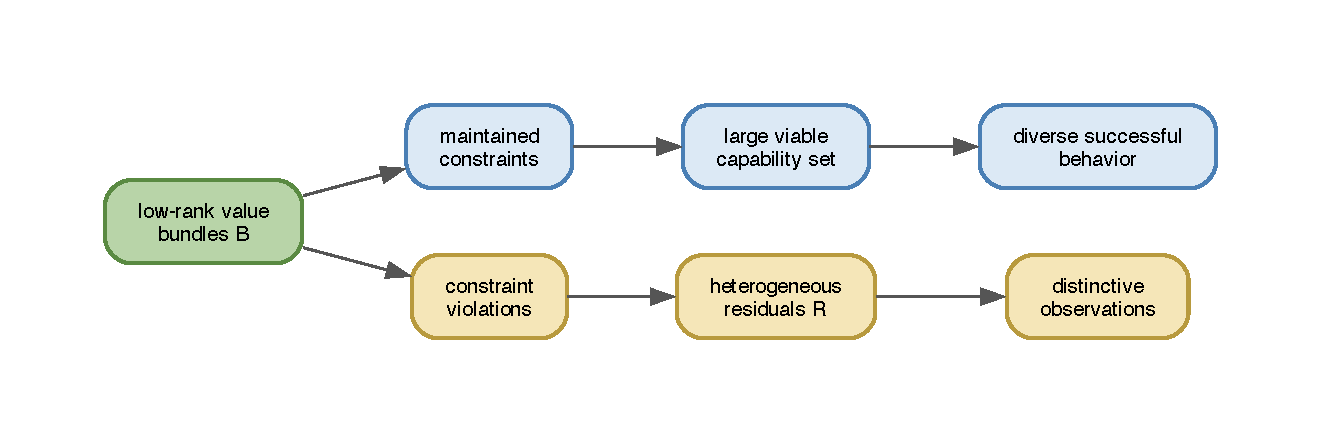
\includegraphics[width=\linewidth]{figures/capability-observability.pdf}
\caption{Capability--observability inversion. Maintained constraints expand the viable action set; constraint violations expand diagnostic residuals.}
\label{fig:capability-observability}
\end{figure}

An observer positioned at the far right sees diverse negative signatures and comparatively undifferentiated normality. A controller positioned at the left may instead be implementing a compact set of invariants whose successful maintenance is what permits behavioral diversity downstream.

\section{Conclusion}

Value inference from behavior should distinguish \emph{what is easy to observe} from \emph{what organizes the system}. Cognitive-ecological research provides a concrete reason for this distinction: positive attributes are often common and similar, while negative attributes are rarer and more diverse, making negative information disproportionately useful for differentiation \citep{AlvesKochUnkelbach2017Common,AlvesKochUnkelbach2018,UnkelbachWeitzelAlves2026}. A control-theoretic interpretation adds a second asymmetry. Successful regulation can maintain a narrow set of invariants while preserving a broad space of feasible trajectories; failures can produce a broad set of diagnostic signatures while destroying options.

The resulting capability--observability inversion suggests a refinement of value-bundle models: high-dimensional behavior is low-rank regulatory bundles plus contextual realization plus high-dimensional failure residuals.
Under this view, the negative side of observed moral and social behavior can be more differentiated without requiring an equally high-dimensional set of fundamental negative values.

For AI value learning, the practical warning is immediate. A learner optimized to extract the most diagnostic features of human behavior may learn the structure of human failures more readily than the structure of human values. The examples that maximize information about identity, group membership, or behavioral prediction need not be the examples that reveal the most causally or normatively important coordinates:
\begin{equation}
    \boxed{
    \arg\max_x I(x;B)
    \neq
    \arg\max_x
    \operatorname{Importance}(x;B).
    }
\end{equation}
Recovering values therefore requires more than observational compression. It requires identifying invariants, interventions, correction dynamics, bearer maps, and the constraints whose successful maintenance preserves the space in which diverse forms of valuable behavior remain possible.

\section*{Acknowledgements}

This manuscript develops ideas from the author's prior work on value bundles \citep{zarncke2026vbd} and viability-constrained value formation \citep{zarncke2026evf}.

\bibliographystyle{plainnat}
\bibliography{value-bundle-inference}

\end{document}
